\documentclass[paper=a4, fontsize=11pt]{scrartcl}
\usepackage[left=1 in, right=1 in, top=1 in, bottom=1 in]{geometry}
\usepackage[T1]{fontenc} 
\usepackage[english]{babel} 
\usepackage{amsmath,amsfonts,amsthm} 
\usepackage[colorlinks]{hyperref}
\usepackage{MnSymbol}
\usepackage{cprotect}
\usepackage{float}
\usepackage[utf8]{inputenc}
\usepackage{sectsty}
\allsectionsfont{ \normalfont\scshape}
\usepackage[document]{ragged2e}
\usepackage{fancyhdr}
\usepackage[dvipsnames]{xcolor}
\usepackage{tikz}
\usepackage{graphicx,subcaption}
\usepackage{setspace}
\graphicspath{ {images/} }
\pagestyle{fancyplain} 
\fancyhead{}
\fancyfoot[L]{} 
\fancyfoot[C]{\thepage}
\fancyfoot[R]{} 
\renewcommand{\headrulewidth}{0pt}
\renewcommand{\footrulewidth}{0pt}
\usepackage{etoolbox}
\patchcmd{\section}{\scshape}{\bfseries}{}{}
\makeatletter
\makeatother
\setlength{\headheight}{10pt}
\numberwithin{figure}{section} 
\numberwithin{table}{section} 
\setlength\parindent{0pt}


\begin{document}

\begin{figure}[H]
\centering
    \begin{subfigure}[b]{\textwidth}
     	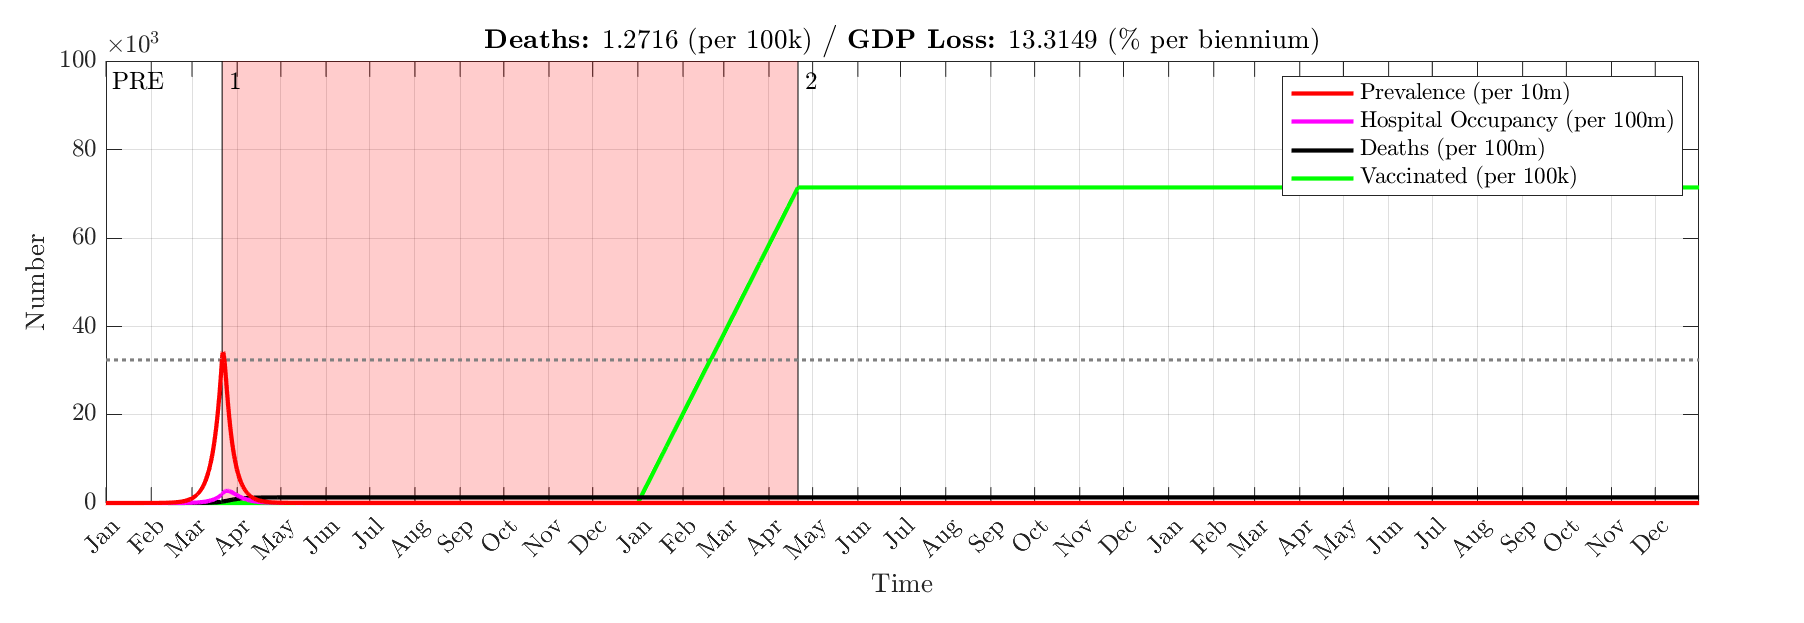
\includegraphics[width=\textwidth,height=5.5cm]{Counterfactuals/UK_swfl}
    \end{subfigure}
    \begin{subfigure}[b]{\textwidth}
      	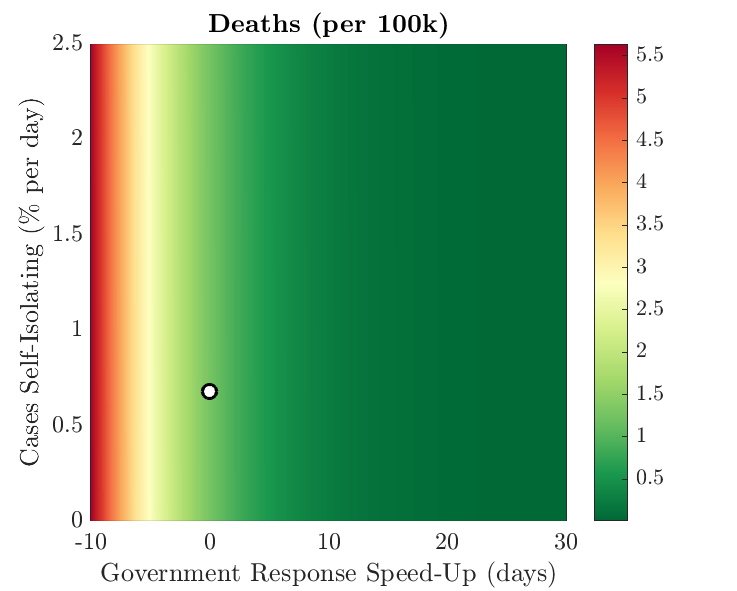
\includegraphics[width=0.49\textwidth,height=6cm]{UK/SWINE/ero_d}
	\hspace{0.05cm}
    	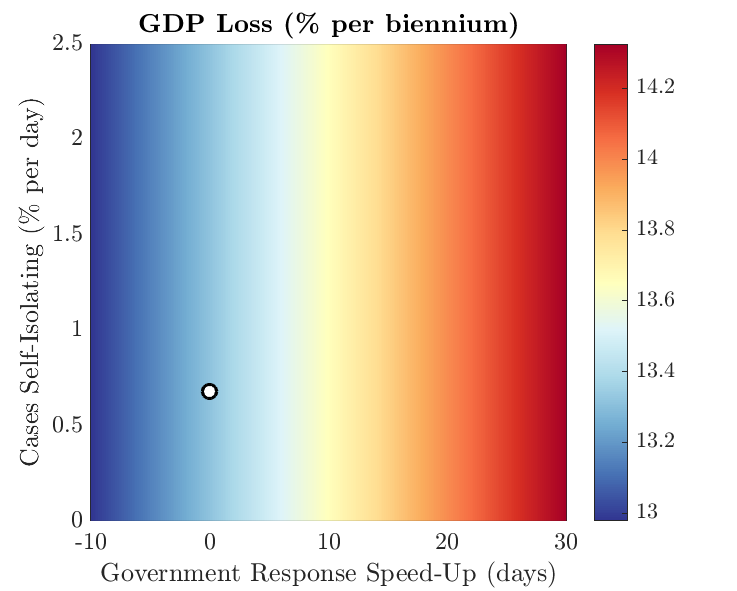
\includegraphics[width=0.49\textwidth,height=6cm]{UK/SWINE/ero_g}
    \end{subfigure}
    \begin{subfigure}[b]{\textwidth}
      	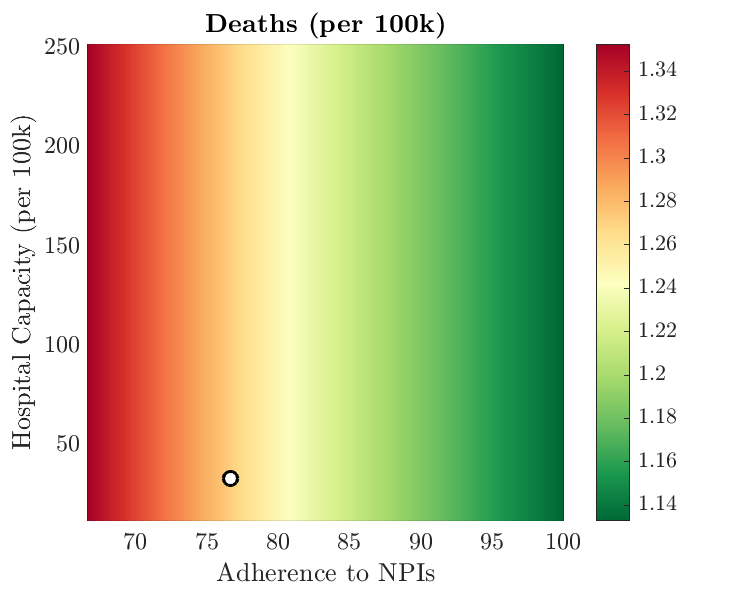
\includegraphics[width=0.49\textwidth,height=6cm]{UK/SWINE/npl_d}
	\hspace{0.05cm}
    	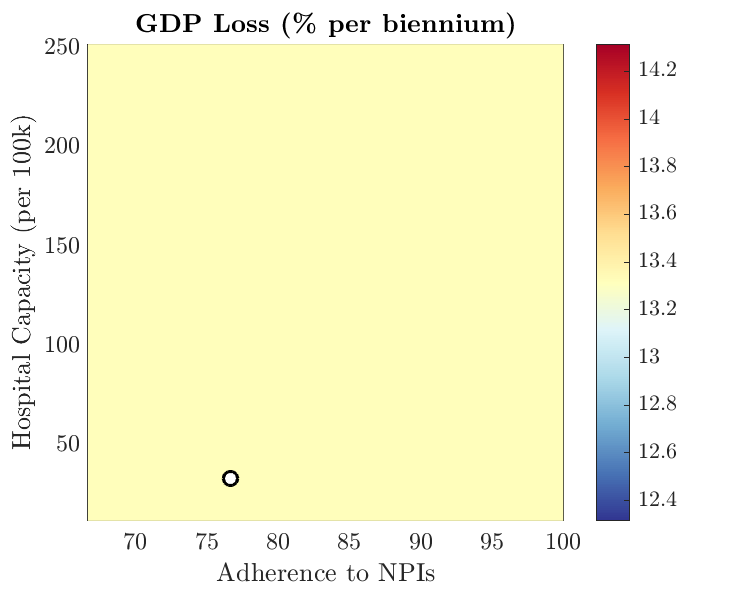
\includegraphics[width=0.49\textwidth,height=6cm]{UK/SWINE/npl_g}
    \end{subfigure}
    \begin{subfigure}[b]{\textwidth}
      	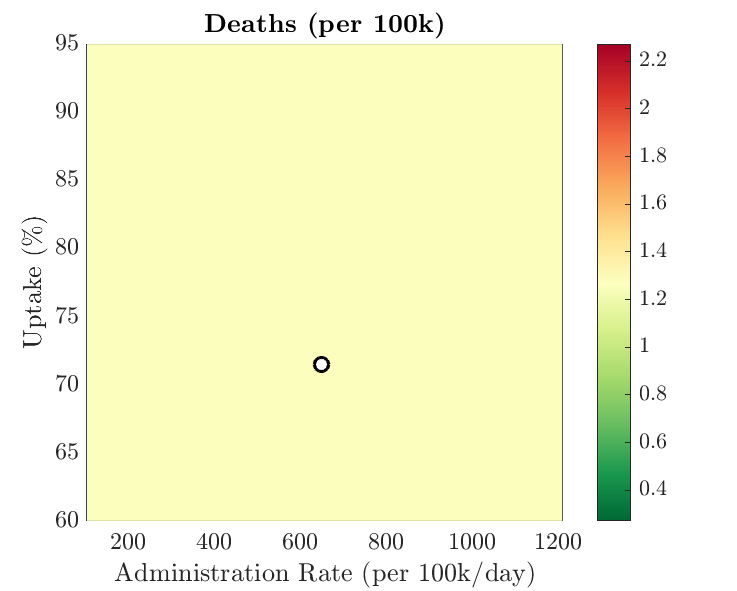
\includegraphics[width=0.49\textwidth,height=6cm]{UK/SWINE/imm_d}
	\hspace{0.05cm}
    	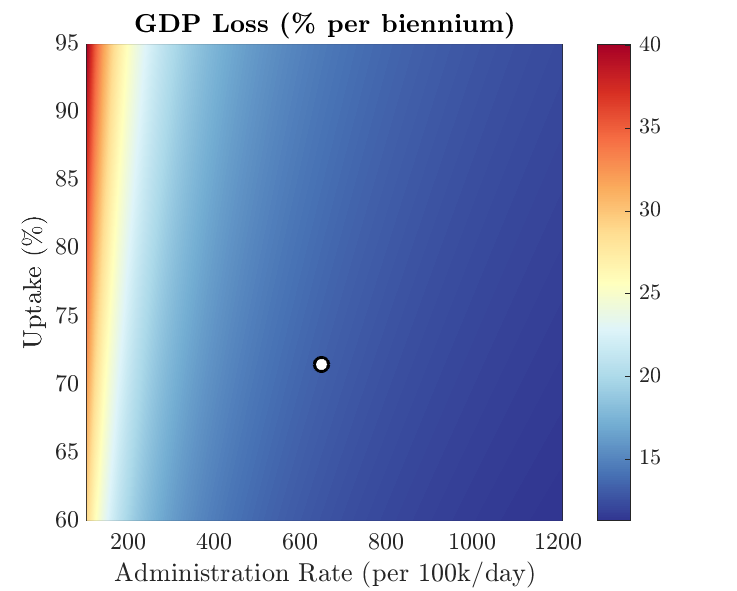
\includegraphics[width=0.49\textwidth,height=6cm]{UK/SWINE/imm_g}
    \end{subfigure}
\caption*{\textbf{Figure 1:} UK} 
\end{figure}

\begin{figure}[H]
\centering
    \begin{subfigure}[b]{\textwidth}
     	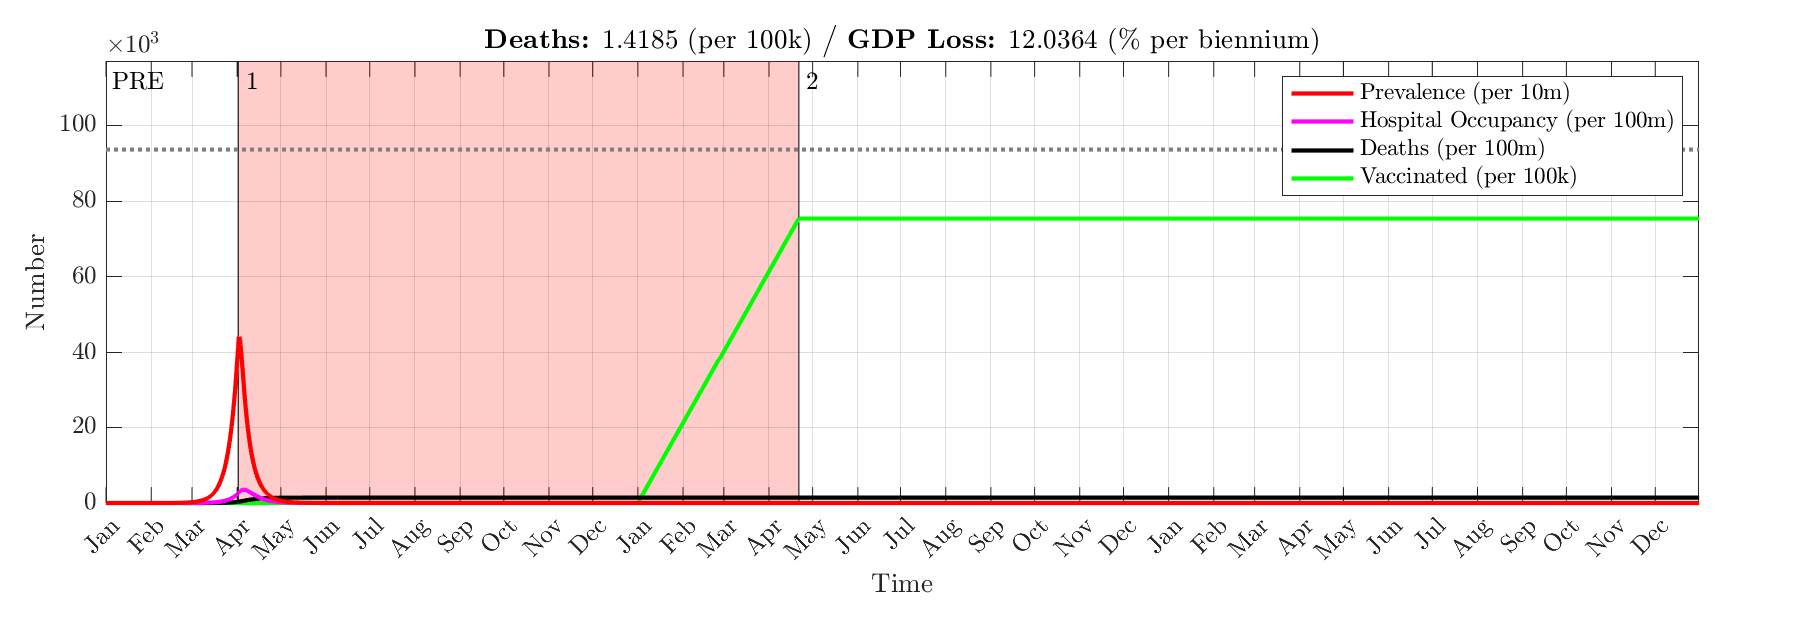
\includegraphics[width=\textwidth,height=5.5cm]{Counterfactuals/US_swfl}
    \end{subfigure}
    \begin{subfigure}[b]{\textwidth}
      	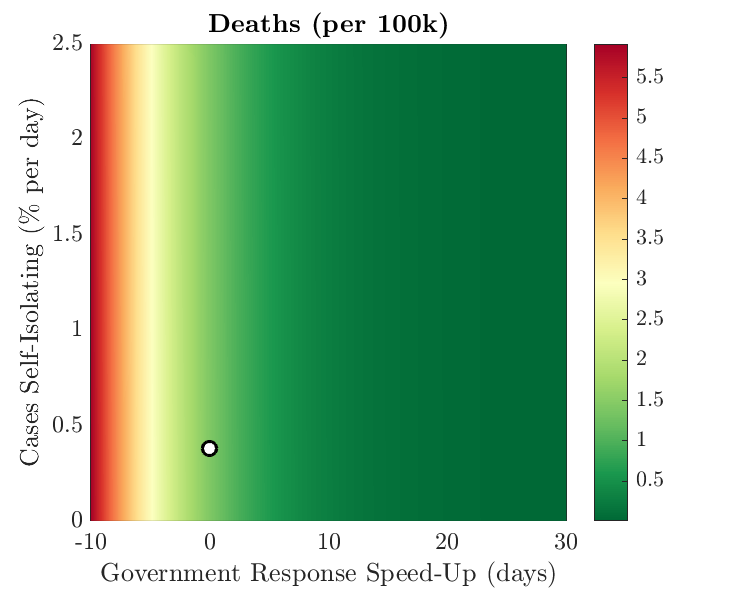
\includegraphics[width=0.49\textwidth,height=6cm]{US/SWINE/ero_d}
	\hspace{0.05cm}
    	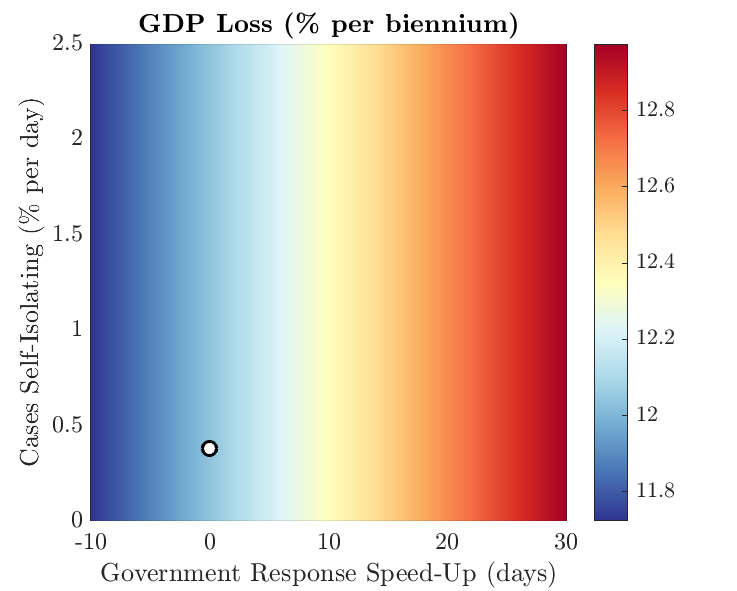
\includegraphics[width=0.49\textwidth,height=6cm]{US/SWINE/ero_g}
    \end{subfigure}
    \begin{subfigure}[b]{\textwidth}
      	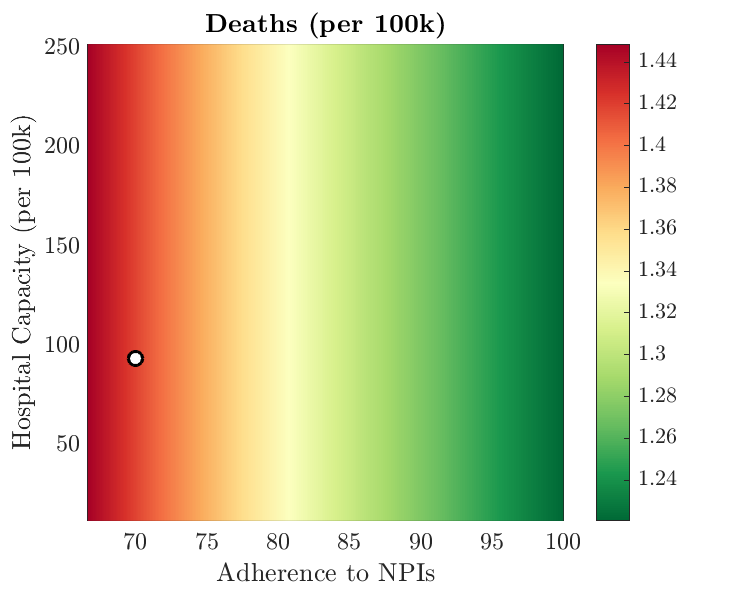
\includegraphics[width=0.49\textwidth,height=6cm]{US/SWINE/npl_d}
	\hspace{0.05cm}
    	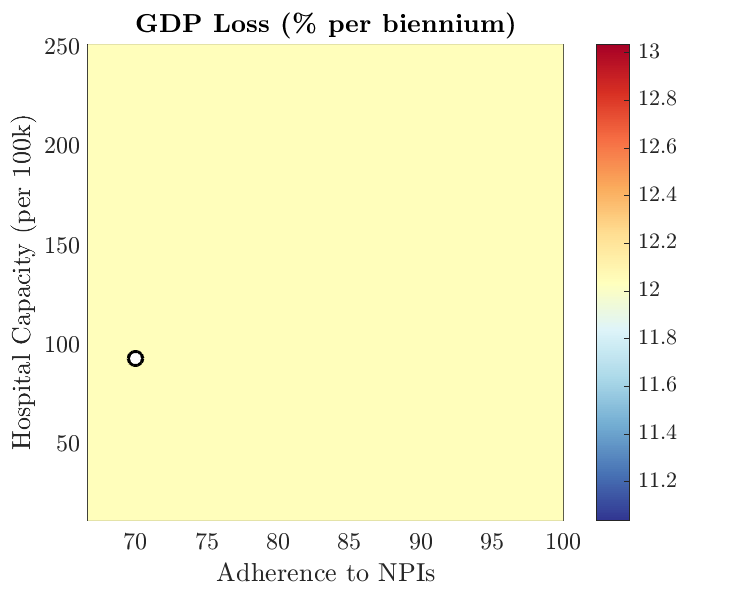
\includegraphics[width=0.49\textwidth,height=6cm]{US/SWINE/npl_g}
    \end{subfigure}
    \begin{subfigure}[b]{\textwidth}
      	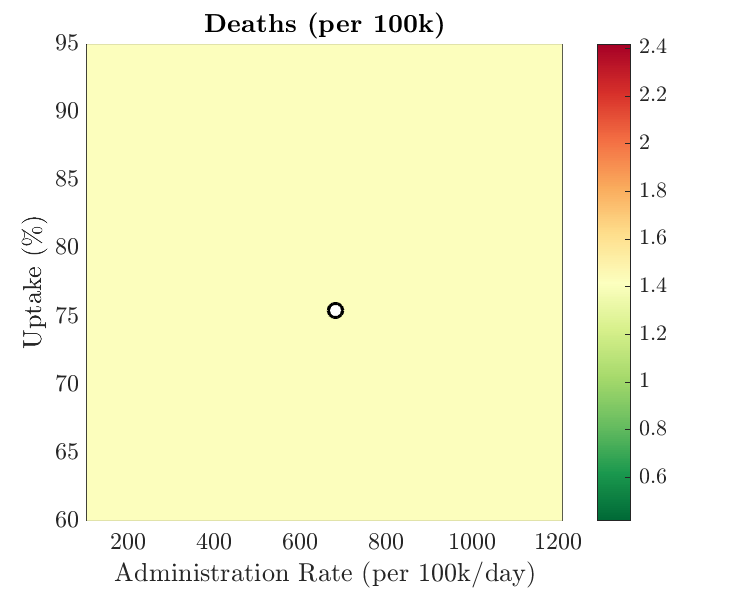
\includegraphics[width=0.49\textwidth,height=6cm]{US/SWINE/imm_d}
	\hspace{0.05cm}
    	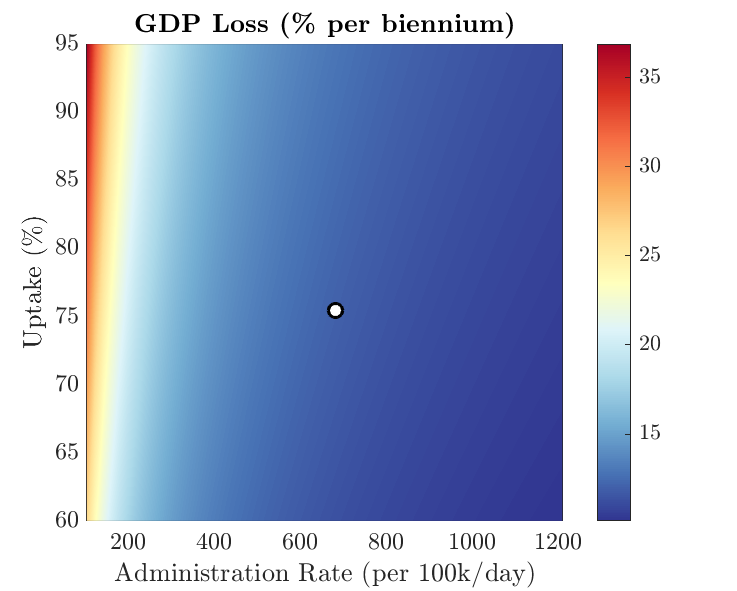
\includegraphics[width=0.49\textwidth,height=6cm]{US/SWINE/imm_g}
    \end{subfigure}
\caption*{\textbf{Figure 2:} US} 
\end{figure}

\begin{figure}[H]
\centering
    \begin{subfigure}[b]{\textwidth}
     	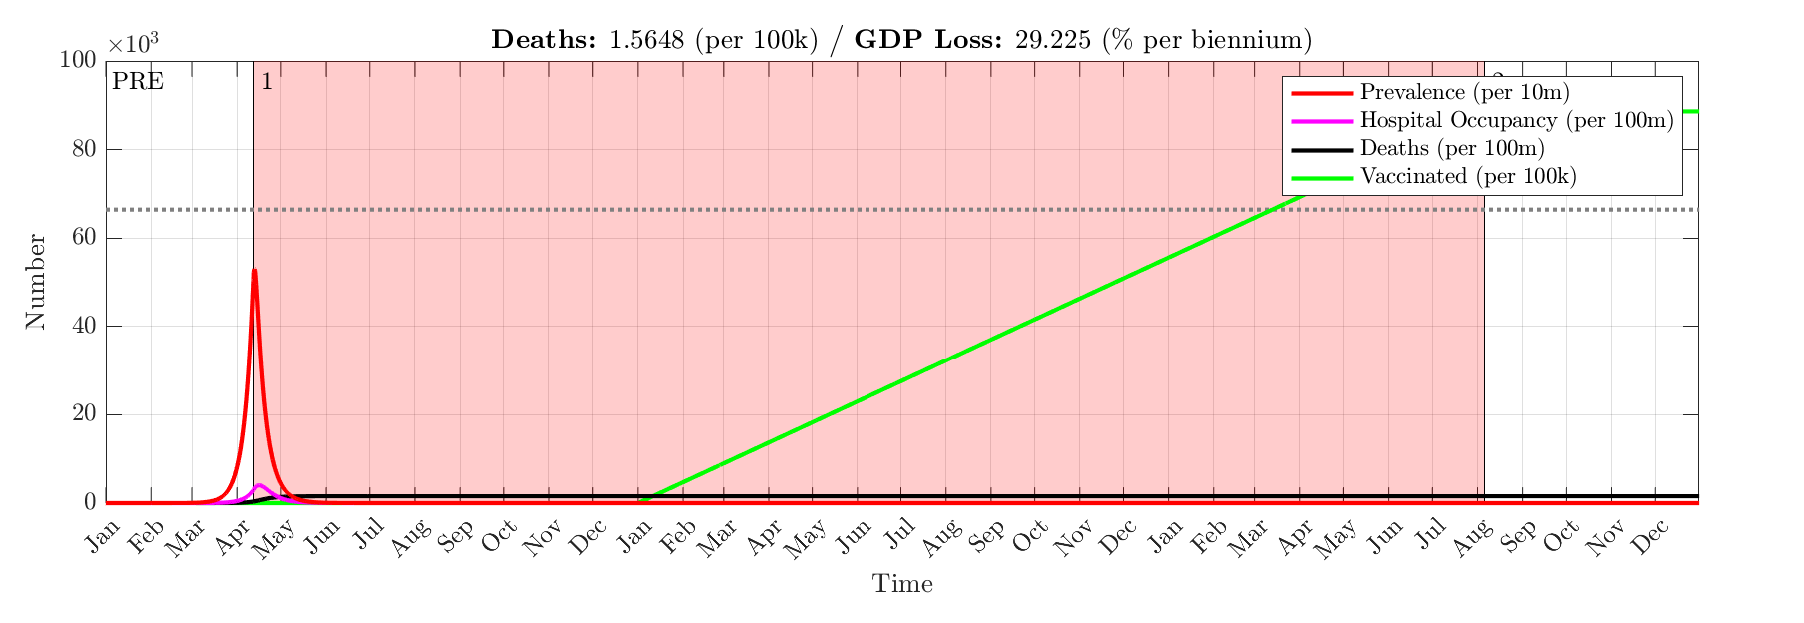
\includegraphics[width=\textwidth,height=5.5cm]{Counterfactuals/CN_swfl}
    \end{subfigure}
    \begin{subfigure}[b]{\textwidth}
      	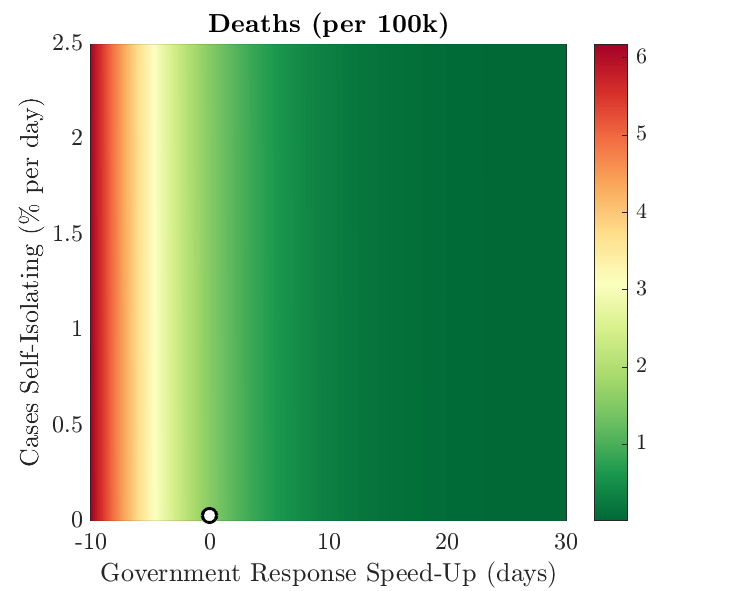
\includegraphics[width=0.49\textwidth,height=6cm]{CN/SWINE/ero_d}
	\hspace{0.05cm}
    	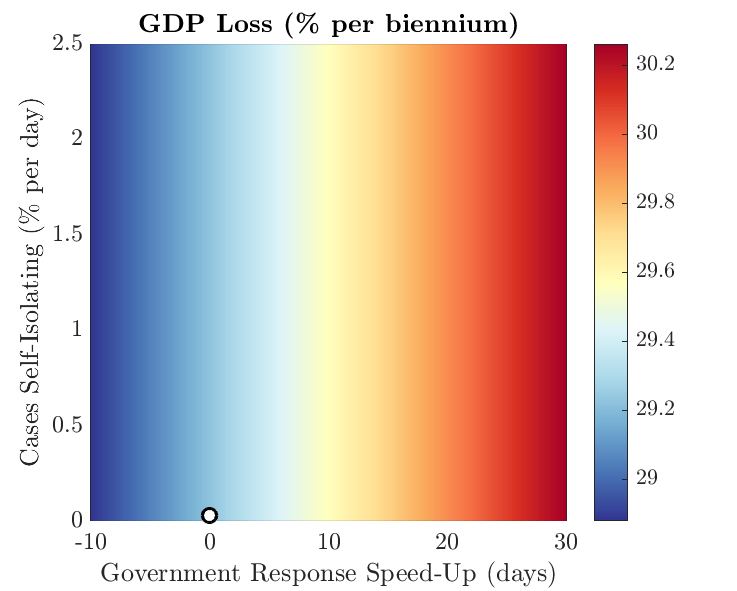
\includegraphics[width=0.49\textwidth,height=6cm]{CN/SWINE/ero_g}
    \end{subfigure}
    \begin{subfigure}[b]{\textwidth}
      	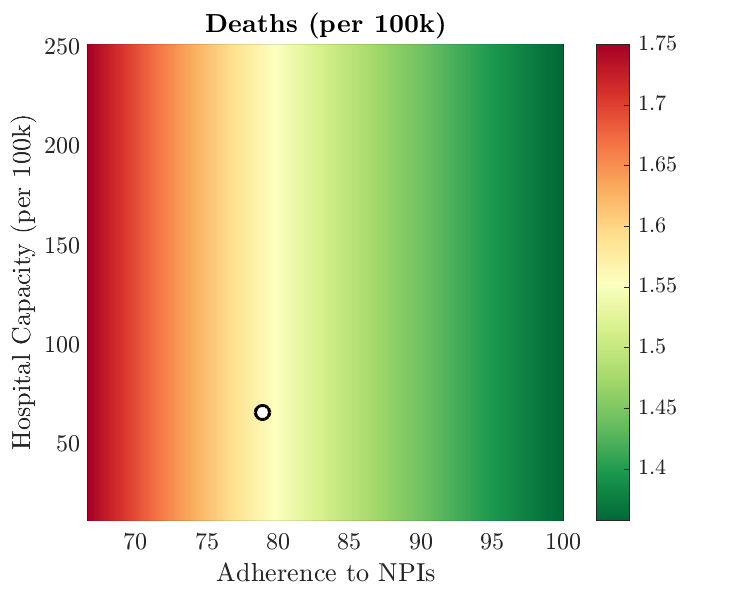
\includegraphics[width=0.49\textwidth,height=6cm]{CN/SWINE/npl_d}
	\hspace{0.05cm}
    	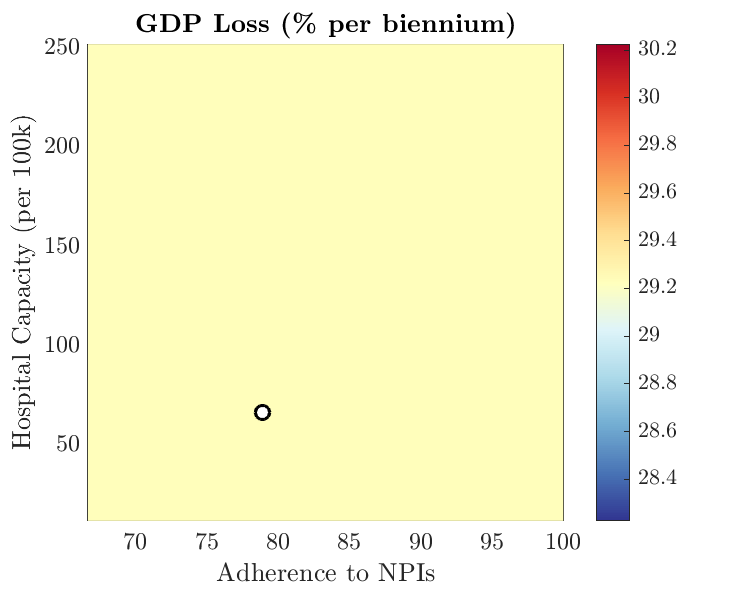
\includegraphics[width=0.49\textwidth,height=6cm]{CN/SWINE/npl_g}
    \end{subfigure}
    \begin{subfigure}[b]{\textwidth}
      	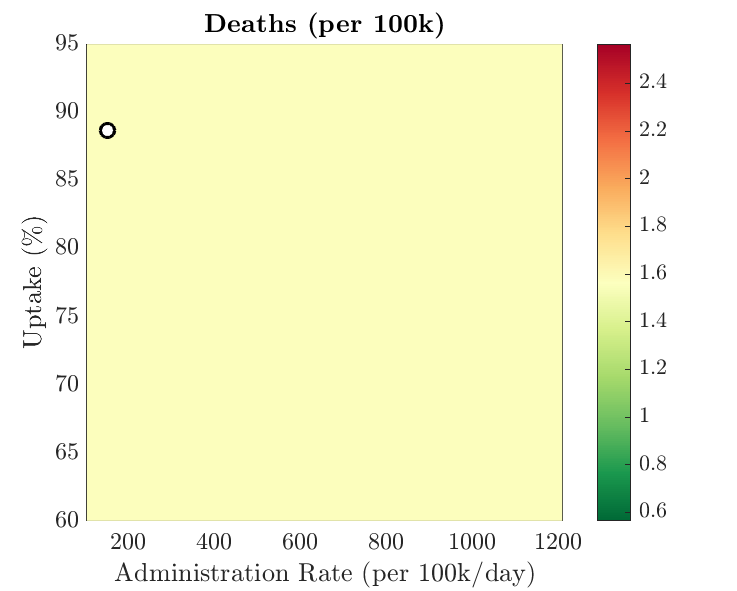
\includegraphics[width=0.49\textwidth,height=6cm]{CN/SWINE/imm_d}
	\hspace{0.05cm}
    	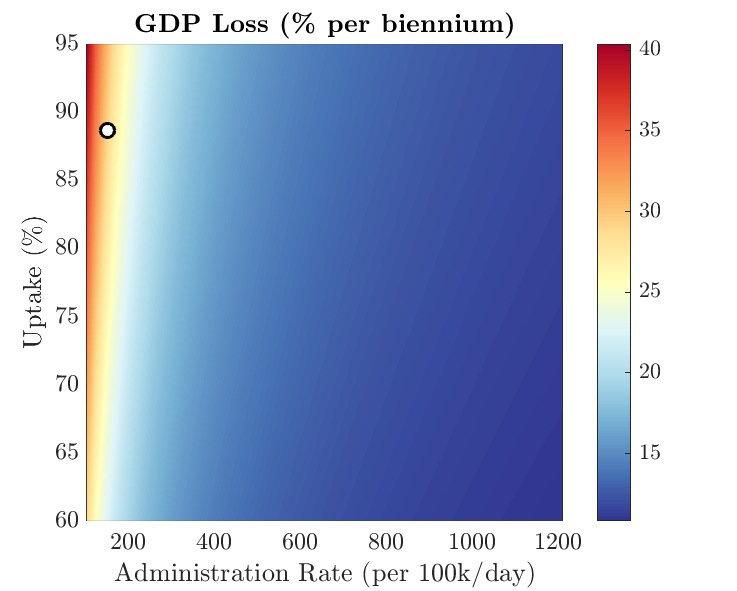
\includegraphics[width=0.49\textwidth,height=6cm]{CN/SWINE/imm_g}
    \end{subfigure}
\caption*{\textbf{Figure 3:} China} 
\end{figure}

\begin{figure}[H]
\centering
    \begin{subfigure}[b]{\textwidth}
     	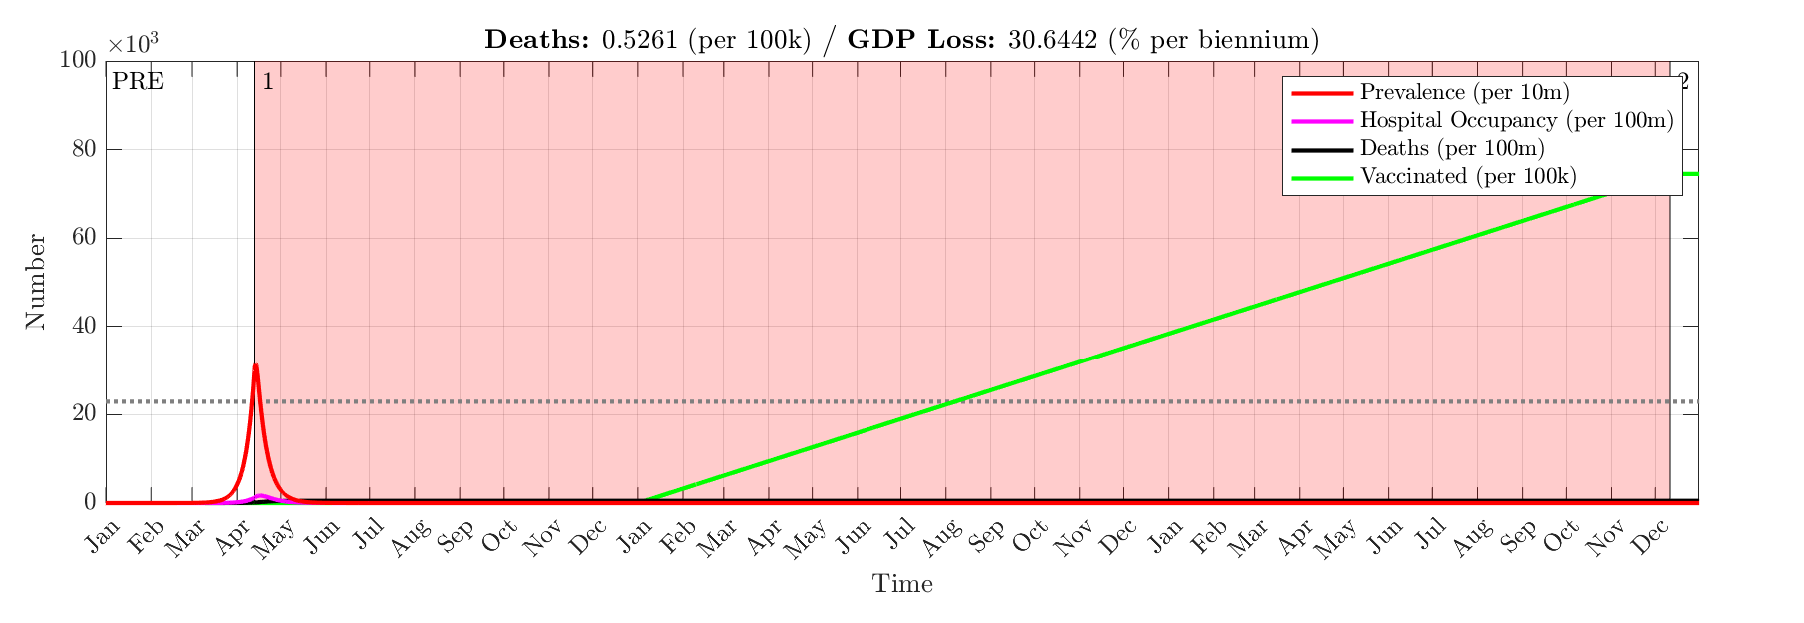
\includegraphics[width=\textwidth,height=5.5cm]{Counterfactuals/IN_swfl}
    \end{subfigure}
    \begin{subfigure}[b]{\textwidth}
      	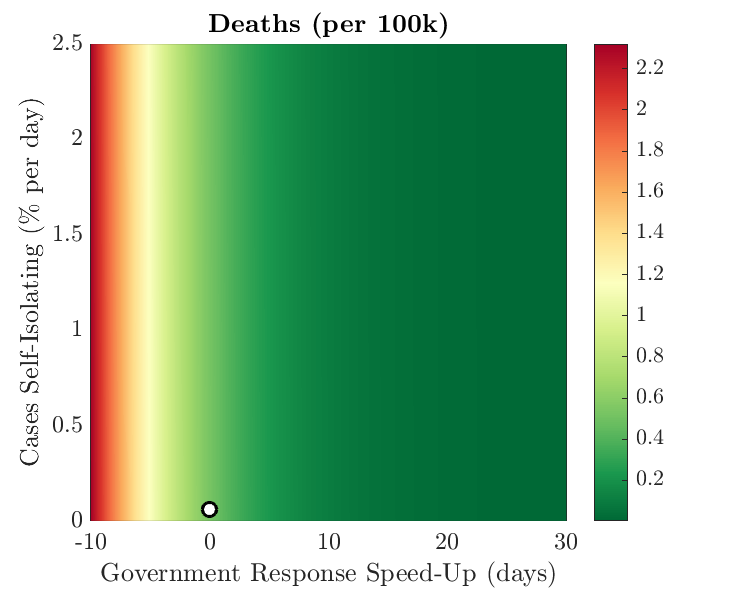
\includegraphics[width=0.49\textwidth,height=6cm]{IN/SWINE/ero_d}
	\hspace{0.05cm}
    	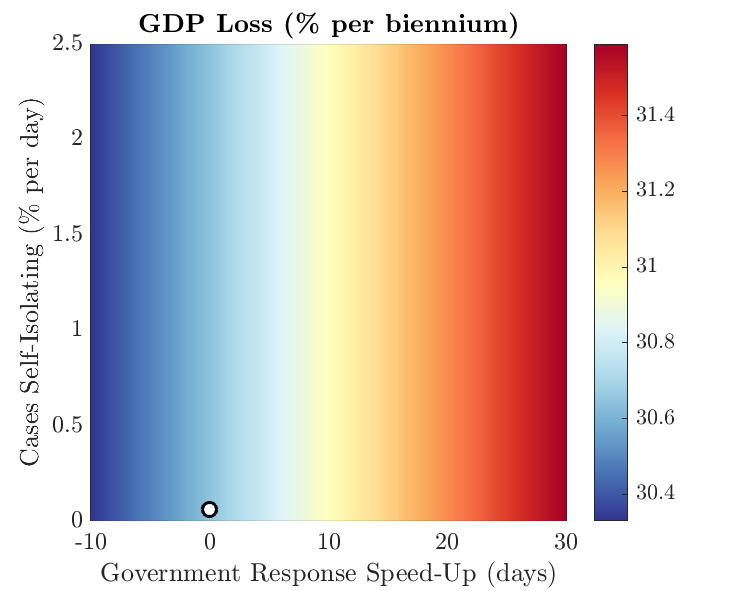
\includegraphics[width=0.49\textwidth,height=6cm]{IN/SWINE/ero_g}
    \end{subfigure}
    \begin{subfigure}[b]{\textwidth}
      	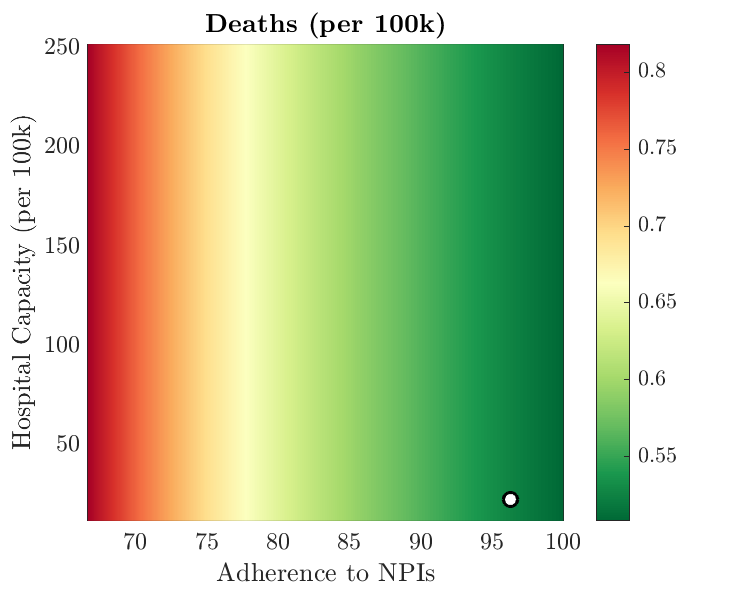
\includegraphics[width=0.49\textwidth,height=6cm]{IN/SWINE/npl_d}
	\hspace{0.05cm}
    	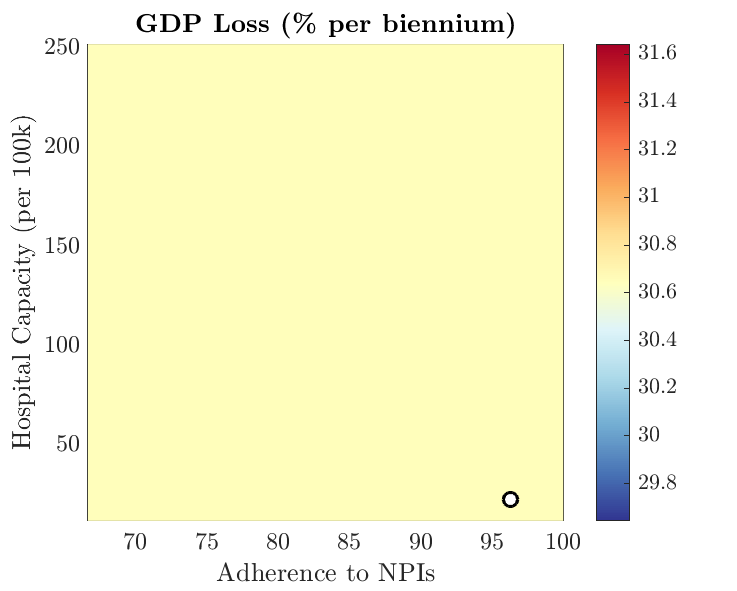
\includegraphics[width=0.49\textwidth,height=6cm]{IN/SWINE/npl_g}
    \end{subfigure}
    \begin{subfigure}[b]{\textwidth}
      	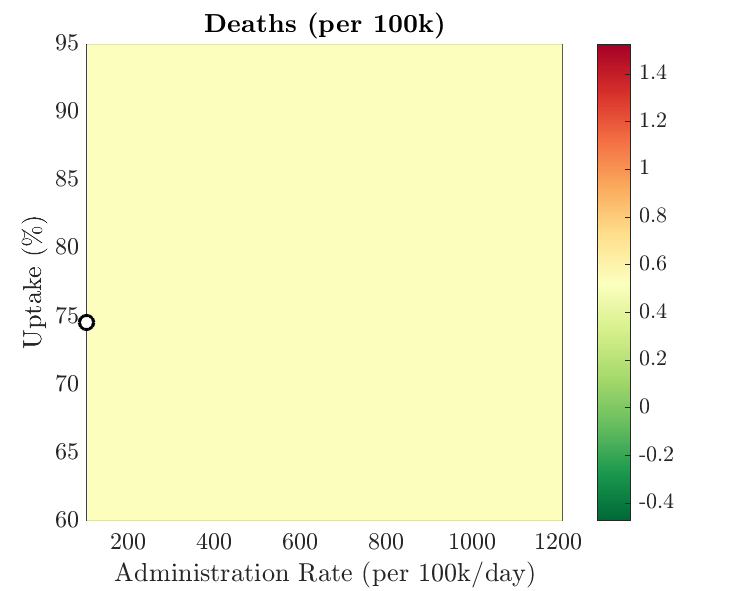
\includegraphics[width=0.49\textwidth,height=6cm]{IN/SWINE/imm_d}
	\hspace{0.05cm}
    	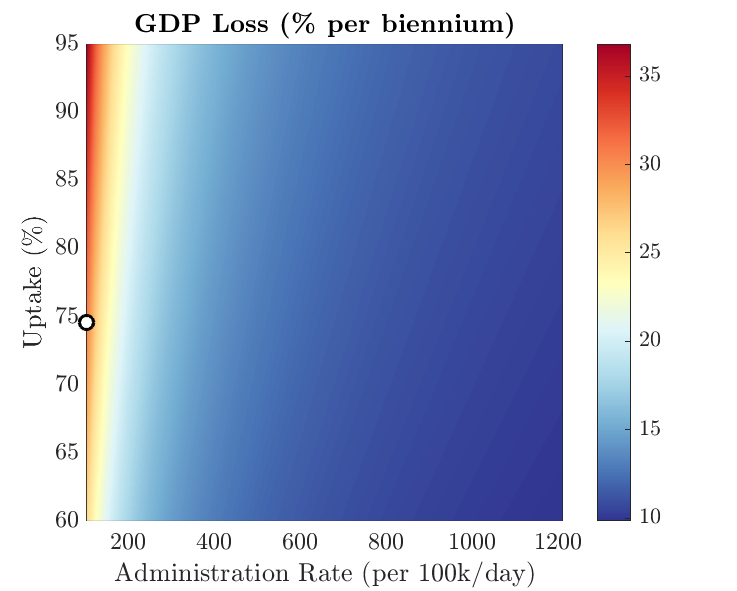
\includegraphics[width=0.49\textwidth,height=6cm]{IN/SWINE/imm_g}
    \end{subfigure}
\caption*{\textbf{Figure 4:} India} 
\end{figure}

\end{document}